\documentclass[11pt,letterpaper]{article}
\usepackage[margin=0.86in]{geometry}
\usepackage[T1]{fontenc}
\usepackage[utf8]{inputenc}
\usepackage{lmodern}
\usepackage{xcolor}
\usepackage{tabularx,booktabs,array,longtable}
\usepackage{enumitem}
\usepackage{hyperref}
\usepackage{fancyhdr}
\usepackage{lastpage}
\usepackage{titlesec}
\usepackage{amsmath,amssymb}
\usepackage{microtype}
\usepackage{graphicx}
\usepackage{listings}
\usepackage{needspace}
\usepackage{ragged2e}
\definecolor{navy}{HTML}{19334C}
\definecolor{teal}{HTML}{236B82}
\definecolor{soft}{HTML}{EFF5F7}
\definecolor{muted}{HTML}{52616B}
\hypersetup{colorlinks=true,linkcolor=teal,urlcolor=teal}
\titleformat{\section}{\Large\bfseries\color{navy}}{\thesection.}{0.6em}{}
\titleformat{\subsection}{\large\bfseries\color{navy}}{\thesubsection}{0.6em}{}
\titleformat{\subsubsection}{\normalsize\bfseries\color{navy}}{\thesubsubsection}{0.6em}{}
\titlespacing*{\section}{0pt}{15pt}{6pt}
\titlespacing*{\subsection}{0pt}{10pt}{4pt}
\setlength{\parindent}{0pt}
\setlength{\parskip}{4.5pt}
\setlength{\headheight}{15pt}
\renewcommand{\arraystretch}{1.16}
\setlist[itemize]{topsep=3pt,itemsep=2pt,leftmargin=1.4em}
\setlist[enumerate]{topsep=3pt,itemsep=2pt,leftmargin=1.5em}
\pagestyle{fancy}
\fancyhf{}
\fancyhead[L]{\small\color{muted} Applied Machine Learning \textbar{} Cornell Tech}
\fancyhead[R]{\small\color{muted} Human or AI?}
\fancyfoot[C]{\small\color{muted} Page \thepage\ of \pageref{LastPage}}
\renewcommand{\headrulewidth}{0.3pt}
\newcommand{\placeholder}[1]{\par\noindent\textcolor{teal}{\textit{[Your response: #1]}}\par\vspace{0.3em}}
\newcommand{\figplaceholder}[1]{\par\noindent\fcolorbox{teal}{soft}{\parbox[c][1.15in][c]{0.94\linewidth}{\centering\textcolor{muted}{Insert #1 here}}}\par}
\newcommand{\question}[2]{\par\needspace{4\baselineskip}\addvspace{0.45em}\noindent\textbf{#1}\quad #2\par\nobreak\vspace{0.1em}}
\newcommand{\smallnote}[1]{{\small\color{muted}#1}}
\newcolumntype{Y}{>{\RaggedRight\arraybackslash}X}

\lstset{basicstyle=\ttfamily\footnotesize,breaklines=true,columns=fullflexible,frame=single}
\newcommand{\FinalTrainAUC}{0.999964}
\newcommand{\FinalValAUC}{0.977012}
\newcommand{\FinalGap}{0.022952}
\newcommand{\FinalThreshold}{0.529366}
\newcommand{\CalSlope}{6.304971}
\newcommand{\CalIntercept}{0.117599}
\newcommand{\FinalFitTime}{12.89}
\newcommand{\Improvement}{0.005784}
\newcommand{\CILow}{0.001478}
\newcommand{\CIHigh}{0.010103}
\newcommand{\PublicScore}{0.92433}
\newcommand{\PrivateScore}{Not yet available}
\newcommand{\SubmissionStatus}{Final selected model: DeBERTa-v3-small; public score confirmed}
\newcommand{\PRLink}{\url{https://github.com/sekhari/human-or-ai-submissions/pull/13}}

\begin{document}
\thispagestyle{empty}
{\color{teal}\bfseries CORNELL TECH | APPLIED MACHINE LEARNING}\par
\vspace{0.2in}
{\Huge\bfseries\color{navy} Human or AI?}\par
\vspace{0.08in}
{\LARGE\color{navy} Group 11: Final Project Report}\par
\vspace{0.2in}
\textbf{Kaggle team:} Group Number 11\par
\textbf{Course GitHub PR:} \PRLink\par
\textbf{Branch:} \texttt{submission/group-number-11}\par
\textbf{Submission status:} \SubmissionStatus\par

\section*{Q0. Team information and model summary}
\question{Q0.1.}{Team members and main contributions.}
\begin{tabularx}{\linewidth}{@{}l l Y@{}}\toprule
Member & NetID & Contributions\\\midrule
Yilin Gao & yg695 & Initial pipeline, model comparison and tuning (Q1); shared split and initial submissions.\\
Ansh Raj Bhargava & ab3396 & Unlabeled-data experiments (Q3) and robustness improvements (Q5).\\
Yingzi Gu (Grace) & yg667 & Learning curves and error analysis (Q2/Q4); final refinement, reproducibility and LaTeX integration, with AI assistance disclosed in Q6.\\\bottomrule
\end{tabularx}\par
\question{Q0.2.}{Final pipeline, from text to probability.}
We concatenate word unigram/bigram TF-IDF and character 3--5-gram TF-IDF. A smoothed class log-count ratio, estimated only from labeled training documents, reweights each feature before fitting a linear SVM with $C=0.5$. We selected this NB-weighted model using the fixed 2,000-row validation set, then retrained it on all 10,000 labeled examples for Kaggle. A sigmoid fitted to full-pipeline out-of-fold training margins converts scores to estimated AI probabilities. The final model does not use pseudo-labels, because the tested self-training candidate had lower validation AUROC.
\question{Q0.3.}{Final scores.}
\begin{tabularx}{\linewidth}{@{}Yr@{}}\toprule
Metric & Score\\\midrule
Selected model validation AUROC & \FinalValAUC\\
Selected model Kaggle public AUROC & \PublicScore\\
Selected model Kaggle private AUROC & \PrivateScore\\\bottomrule
\end{tabularx}\par
\smallnote{The only screenshot-confirmed earlier public score is 0.85049 for \texttt{submission\_word\_svm\_c05.csv}. It is not the score of the selected NB-weighted model. No private score is inferred or fabricated.}

\smallnote{All experiments use the committed 8,000/2,000 split and seed 42. No raw or case/whitespace-normalized exact cross-split duplicates were found; near duplicates were not exhaustively tested. Repeated selection can make validation scores optimistic.}

\newpage
\section*{Q1. Model comparison and selection}
\question{Q1.1.}{Preprocessing and text representation.}
We use light preprocessing to preserve stylistic cues. The word vectorizer lowercases text and uses scikit-learn's default word-token pattern (tokens of at least two word characters), with unigrams and bigrams. Character features use lowercased character 3--5-grams and retain local punctuation and spacing patterns. Both vectorizers use minimum document frequency 2, sublinear term frequency, their default smoothed IDF and L2 normalization, with caps of 100,000 word and 150,000 character features. Each vocabulary and its IDF weights are learned exclusively from training data. Character features complement vocabulary with morphology and local formatting. The final model adds supervised NB feature weighting, defined in Q5; it does not apply the Unicode folding tested in the robustness experiment.
\question{Q1.2.}{Comparison of three modeling approaches on the same split.}
\par\noindent
\begin{tabularx}{\linewidth}{@{}Yrrr@{}}
\toprule
Model (word TF-IDF) & Train AUC & Val. AUC & Fit (s) \\
\midrule
Linear SVM ($C=1$) & 1.000000 & 0.943355 & 2.16 \\
Logistic regression ($C=1$) & 0.995359 & 0.934601 & 2.14 \\
Complement NB ($\alpha=1$) & 0.984366 & 0.896508 & 1.91 \\
\bottomrule
\end{tabularx}
\par

\smallnote{Current-environment rerun. All three use word TF-IDF; timing includes feature extraction and classifier fitting, excluding evaluation. Historical teammate results are retained separately and differ slightly because the original environment was not pinned.}
\question{Q1.3.}{Hyperparameters for at least two approaches and selection protocol.}
For logistic regression we searched $C\in\{0.1,0.5,1,2,5\}$; for the linear SVM, $C\in\{0.01,0.1,0.5,1,2\}$. All other settings and validation IDs were fixed. The best word-only values were $C=5$ and $C=0.5$, respectively. We selected by held-out AUROC without test labels. Full results are below; this is model selection on a reused holdout rather than an unbiased final test estimate.
{\small\par\noindent
\begin{tabularx}{\linewidth}{@{}Yrrr@{}}
\toprule
Model & $C$ & Train AUC & Val. AUC \\
\midrule
Logistic Regression & 0.1 & 0.959492 & 0.908819 \\
Logistic Regression & 0.5 & 0.986518 & 0.928824 \\
Logistic Regression & 1 & 0.995359 & 0.934601 \\
Logistic Regression & 2 & 0.999386 & 0.939157 \\
Logistic Regression & 5 & 0.999999 & 0.942735 \\
Linear SVM & 0.01 & 0.956640 & 0.905830 \\
Linear SVM & 0.1 & 0.995047 & 0.935096 \\
Linear SVM & 0.5 & 1.000000 & 0.943666 \\
Linear SVM & 1 & 1.000000 & 0.943355 \\
Linear SVM & 2 & 1.000000 & 0.942228 \\
\bottomrule
\end{tabularx}
\par
}
\question{Q1.4.}{Final selection and subsequent changes.}
The original selected model combined word and character TF-IDF with SVM $C=0.5$, reaching 0.971228 in the current environment. We then compared six fixed refinement configurations (Q5). NB-weighted TF-IDF achieved \FinalValAUC, a gain of \Improvement, with similar laptop-scale training cost, and was selected. Its label-dependent feature weights are refitted within every calibration fold. We retained the original supervised model for Q2's controlled learning-curve experiment, but reran all Q4 analyses on the final selected model. Q3 and Q5 negative results remain part of the experimental record rather than being overwritten.

\newpage
\section*{Q2. Effect of training data size}
\question{Q2.1.}{One fixed configuration at five training sizes.}
We use the original word + character TF-IDF / SVM ($C=0.5$) configuration throughout this experiment. This is the supervised reference configuration, not the later NB-weighted final model. Using seed 42, we independently shuffle each class pool and interleave them to obtain balanced, nested training subsets. The 8,000-row fit retains the original committed row order. Every size refits its own vocabulary and IDF weights, with identical hyperparameters and the same untouched validation IDs.

\par\noindent
\begin{tabularx}{\linewidth}{@{}Yrrr@{}}
\toprule
Training rows & Train AUC & Val. AUC & Fit (s) \\
\midrule
500 & 1.000000 & 0.890672 & 0.63 \\
1,000 & 1.000000 & 0.923734 & 1.28 \\
2,000 & 1.000000 & 0.947738 & 2.62 \\
5,000 & 1.000000 & 0.965055 & 6.26 \\
8,000 & 1.000000 & 0.971228 & 9.77 \\
\bottomrule
\end{tabularx}
\par

\smallnote{Times include TF-IDF and SVM fitting, excluding scoring and probability calibration. Subset membership is recorded in \texttt{learning\_curve\_subset\_ids.csv}.}
\question{Q2.2.}{Learning curve.}
\begin{center}
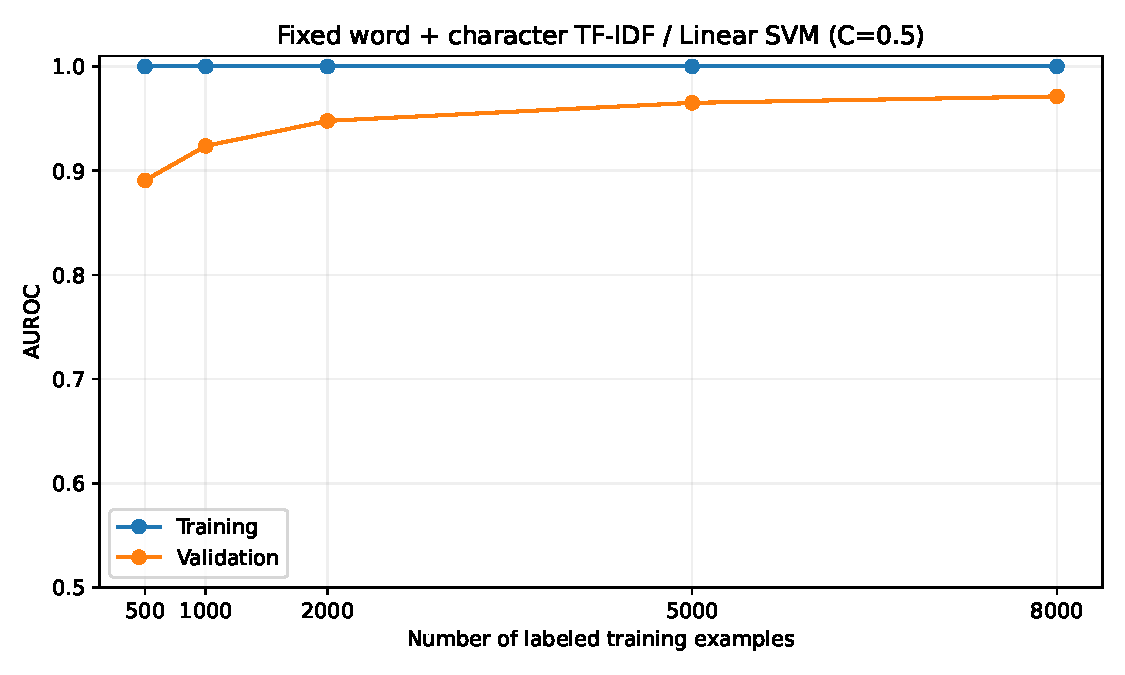
\includegraphics[width=0.78\linewidth]{figures/learning_curve.pdf}
\end{center}
\question{Q2.3.}{Overfitting, underfitting and the value of more labels.}
Training AUROC is 1.0 at every size, while validation AUROC increases monotonically from 0.890672 to 0.971228. The initial gap of 0.109328 is consistent with overfitting in a high-dimensional representation, not an inability to fit the training observations. The gap falls to 0.028772 at 8,000 rows. There are diminishing returns: adding 3,000 examples from 2,000 to 5,000 improves validation AUROC by 0.017317; adding another 3,000 improves it by 0.006173. More labels from a similar distribution therefore appear useful, but this single seeded curve does not establish uncertainty or the gain beyond 8,000 examples. Additional in-distribution data may also fail to address unseen domains or adversarial editing.

\newpage
\section*{Q3. Learning from unlabeled data}
\question{Q3.1.}{Method and leakage prevention.}
Person B tested confidence-based self-training using the 3,000 unlabeled passages. The supervised word + character SVM predicts margins, transformed to probabilities with a logistic sigmoid fitted to five-fold out-of-fold training margins. Passages with estimated AI probability at least $t$ or at most $1-t$ receive pseudo-labels and are added to training. Thresholds $t\in\{0.99,0.95,0.90,0.80,0.50\}$ were compared, followed by up to three rounds at the best threshold. Vectorizer fitting, calibration, and pseudo-label generation exclude the fixed validation set. Validation labels select settings but do not train models. These exploratory calibration folds share a vocabulary fitted on the 8,000-row training partition; the revised final-refinement implementation instead refits the full pipeline per fold.
\question{Q3.2.}{Supervised versus unlabeled-data results.}
\par\noindent
\begin{tabularx}{\linewidth}{@{}Yrrr@{}}
\toprule
Method & Pseudo rows & Val. AUC & Time (s) \\
\midrule
Supervised baseline & 0 & 0.971122 & 64.85 \\
Fit TF-IDF on training + unlabeled & 0 & 0.971217 & 89.17 \\
One round; confidence 0.99 & 1118 & 0.971113 & 75.49 \\
One round; confidence 0.95 & 1849 & 0.971640 & 75.44 \\
One round; confidence 0.9 & 2167 & 0.972072 & 75.65 \\
One round; confidence 0.8 & 2479 & 0.972052 & 75.14 \\
One round; confidence 0.5 & 3000 & 0.971796 & 75.32 \\
self-training round 1; confidence 0.9 & 2167 & 0.972072 & 75.10 \\
self-training round 2; confidence 0.9 & 2239 & 0.972232 & 87.93 \\
self-training round 3; confidence 0.9 & 2255 & 0.972122 & 100.66 \\
\bottomrule
\end{tabularx}
\par

\smallnote{Person B's committed Kaggle-environment results, preserved without replacing them with another environment's numbers. Runtime includes feature preparation; later self-training rounds report cumulative runtime. The current-environment reference AUROC is 0.971228 versus historical 0.971122.}
\question{Q3.3.}{Did it help, and what limits the conclusion?}
Self-training helped modestly: the best recorded two-round result was 0.972232 versus 0.971122 for supervised learning, a gain of 0.001110. At threshold 0.90, the first round added 2,167 pseudo-labeled passages; the second added 2,239. Lower thresholds admit more data but can introduce noise. In a training-only simulation, threshold 0.90 selected 2,022 of 3,000 held-back labeled examples with 1.88\% error, compared with 9.6\% when all were selected. This is an optimistic in-distribution diagnostic, not the error rate on genuinely unlabeled data. Threshold and round selection reuse the validation set, so the small gain is not independent confirmatory evidence.

\subsection*{Connection to final refinement}
We also evaluated a reproducible two-round candidate with threshold 0.90 and a frozen sigmoid fitted from three-fold, full-pipeline out-of-fold training scores. Freezing avoids recalibrating on folds that contain pseudo-labels generated using all training targets. This revised procedure obtained 0.972186, above the current supervised baseline but below NB weighting. It differs from Person B's procedure and is reported as a separate experiment, not an exact reproduction. Its pseudo-label counts were 2,171 and 2,254. The final selected model therefore remains supervised.

\newpage
\section*{Q4. Generalization and error analysis}
\question{Q4.1.}{Training versus validation performance of the final model.}
The final NB-weighted model achieved training AUROC \FinalTrainAUC\ and validation AUROC \FinalValAUC, a gap of \FinalGap. This suggests some overfitting, while held-out ranking remains strong. High dimensionality, residual differences between training and validation passages, and repeated validation-based model selection are plausible contributors. No single cause is established. AUROC describes ranking, not accuracy at a fixed threshold. At the original SVM decision threshold of margin zero, the confusion matrix is:

\par\noindent
\begin{tabularx}{\linewidth}{@{}Yrr@{}}
\toprule
True class & Predicted human & Predicted AI \\
\midrule
Human & 944 & 56 \\
AI & 106 & 894 \\
\bottomrule
\end{tabularx}
\par


There are 56 false positives and 106 false negatives: false-positive rate 5.6\%, false-negative rate 10.6\%, and accuracy 91.9\%. The original unweighted model had 50 false positives and 127 false negatives, so improved ranking did not reduce both error types at the unchanged threshold.
\question{Q4.2.}{Observable subgroups and differences.}
We group passages by whitespace-separated word count, an observable quantity requiring no hidden domain information. The training length tertiles, 175 and 240 words, define short ($\leq175$), medium (176--240), and long ($>240$) groups. Ties stay together; boundaries were not chosen to maximize validation scores.

\par\noindent
\begin{tabularx}{\linewidth}{@{}Yrrrr@{}}
\toprule
Group (words) & Count & Human / AI & Val. AUC & FP / FN \\
\midrule
Short (76--175) & 711 & 352 / 359 & 0.970135 & 29 / 38 \\
Medium (176--240) & 643 & 355 / 288 & 0.981289 & 22 / 27 \\
Long (241--350) & 646 & 293 / 353 & 0.983670 & 5 / 41 \\
\bottomrule
\end{tabularx}
\par


Short texts have the lowest AUROC (0.970135), while medium and long texts reach 0.981289 and 0.983670. Longer passages may provide more lexical and stylistic evidence, but this is an association, not a causal effect: topic, genre and class composition also differ. The long group still contains 41 false negatives at the fixed threshold. Group AUROC and threshold-dependent error counts should therefore be interpreted separately. Counts are included to show the amount of evidence behind each group.

\subsection*{Probability estimates and operating point}
We refit the entire NB-weighted pipeline in each of three stratified training folds and fit a logistic sigmoid to its out-of-fold margins. The held-out validation set never enters calibration. The fitted transformation is
\[
\widehat P(\mathrm{AI}\mid s)=\operatorname{sigmoid}(\CalSlope\,s+\CalIntercept).
\]
We retain the SVM's decision rule $s>0$, equivalent to $\widehat P(\mathrm{AI})>\FinalThreshold$. This is not a probability threshold of 0.5. The increasing transformation preserves AUROC; its probabilities may still be imperfectly calibrated because fold models use fewer observations than the full fit. The final Kaggle pipeline separately recalibrates using out-of-fold scores from all 10,000 labeled examples.

\newpage
\section*{Q4. Error examples and interpretation (continued)}
\question{Q4.3.}{Five false positives and five false negatives.}
FP means human text predicted AI; FN means AI text predicted human. We inspect the five highest-margin FP and five lowest-margin FN, deliberately emphasizing confident failures. These examples are not a random or representative sample of all errors. Reasons below are hypotheses grounded in passage inspection, not proven feature attributions or a claim that dataset labels are wrong.

{\small\renewcommand{\arraystretch}{1.12}\par\noindent
\begin{tabularx}{\linewidth}{@{}rrrY@{}}
\toprule
ID & Error & P(AI) & Observed features / possible failure \\
\midrule
3671 & FP & 0.975171 & Polished human biography: third-person facts and institutional names overlap with generated exposition. \\
3326 & FP & 0.972815 & Human film review: formulaic praise and plot/cast/music structure resemble generated reviews. \\
3448 & FP & 0.962793 & Human technical reference: repeated terminology and explanatory prose may receive AI-associated weights. \\
4587 & FP & 0.914680 & Human forum question: structured hypothetical reasoning and repetition resemble generated explanations. \\
6567 & FP & 0.910239 & Human historical summary: dates, named organizations, and broad concluding statements mimic AI summaries. \\
1524 & FN & 0.000124 & AI abstract plus personal question: technical terminology and missing visual context imitate a copied forum discussion. \\
3062 & FN & 0.002571 & AI personal narrative: greetings, uncertainty, awkward wording, and personal detail imitate human forum writing. \\
8986 & FN & 0.002896 & AI recipe: ingredient lists and headings mimic human recipes; an incongruous personal ending is overlooked. \\
2209 & FN & 0.010841 & AI recipe: quantities and ordinary procedural verbs resemble human instructions, with no obvious local anomaly. \\
3665 & FN & 0.021416 & AI news-style passage repeats one claim extensively. Topic cues dominate; sublinear TF and normalization dampen repetition. \\
\bottomrule
\end{tabularx}
\par
}

\question{Q4.4.}{Recurring failure patterns and a targeted response.}
Polished human reference prose and reviews can resemble AI exposition (3671, 3326, 3448, 6567), while AI imitates technical forum posts, personal narratives, and recipes (1524, 3062, 8986, 2209). Genre and presentation therefore provide ambiguous authorship cues. Example 3665 adds a distinct failure: a news-style passage repeats nearly the same sentence throughout. Local lexical features preserve news vocabulary, while sublinear term frequency and normalization dampen repetition; the representation does not explicitly encode duplicate-sentence frequency. A targeted next experiment would add sentence-duplication fraction and longest repeated-sentence run as training-derived features, then compare against the unchanged baseline on the fixed validation IDs. This proposal has not been tested here. The selected cases support hypotheses but do not estimate prevalence, and neither surface polish nor factual plausibility establishes authorship.

\newpage
\section*{Q5. Open-ended improvements and insights}
\question{Q5.1.}{Hypotheses motivating improvements.}
Person B hypothesized that Unicode folding and typo augmentation could reduce brittleness to edited AI text, as the assignment describes adversarially modified test passages. Word/character TF-IDF matches local forms, so visually similar characters or inserted invisible characters may change features. In a later refinement, we hypothesized that class-informed feature weighting could emphasize discriminative word and character patterns instead of treating TF-IDF dimensions equally before regularization. These are separate experiments: robustness is evaluated on both original and synthetically perturbed validation passages, whereas final selection uses the original fixed validation set. Neither hypothesis guarantees improvement on the hidden test distribution.
\question{Q5.2.}{Changes and controlled comparisons.}
For robustness, R0 is word-only SVM; R1 is the word + character baseline; R2 adds NFKC normalization, selected homoglyph folding, zero-width removal and whitespace normalization; R3 additionally augments both training classes with typos. All retain SVM $C=0.5$ and the fixed split. The stress tests perturb only AI-labeled validation passages using typos, Cyrillic look-alikes, or inserted zero-width characters; they are synthetic conditions, not known test-set memberships.

For refinement, we specified six candidates: baseline, character weight 2, character-only features, logistic regression $C=5$, NB weighting, and revised two-round self-training. With binary training-document occurrence counts $n_{cj}$ for class $c$ and feature $j$, NB weighting uses
\[
p_{cj}=\frac{1+n_{cj}}{\sum_k(1+n_{ck})},\qquad
r_j=\log\frac{p_{1j}}{p_{0j}},\qquad x'_j=x_jr_j.
\]
The same word/character TF-IDF settings and SVM $C=0.5$ are retained. Counts use training labels only and are refitted within calibration folds. Validation labels never define $r_j$.
\question{Q5.3.}{Measured results.}
{\small\par\noindent
\begin{tabularx}{\linewidth}{@{}Yrrrrr@{}}
\toprule
Configuration & Original & Typos & Homoglyph & Zero-width & Fit (s) \\
\midrule
R0 & 0.9433 & 0.9404 & 0.9027 & 0.9185 & 5.12 \\
R1 & 0.9711 & 0.9696 & 0.9578 & 0.9600 & 28.53 \\
R2 & 0.9597 & 0.9576 & 0.9597 & 0.9597 & 28.94 \\
R3 & 0.9590 & 0.9573 & 0.9590 & 0.9590 & 53.96 \\
\bottomrule
\end{tabularx}
\par
}
\smallnote{Historical Person B run. All score columns are validation AUROC; original means unmodified validation. Runtime includes feature extraction and fitting.}

\vspace{0.1in}
{\small\par\noindent
\begin{tabularx}{\linewidth}{@{}Yrrr@{}}
\toprule
Candidate & Train AUC & Val. AUC & Fit (s) \\
\midrule
Original word + character SVM & 1.000000 & 0.971228 & 9.80 \\
Character block weighted 2x & 1.000000 & 0.971349 & 9.78 \\
Character-only SVM & 0.999978 & 0.969718 & 8.27 \\
Word + character logistic regression & 1.000000 & 0.969331 & 12.05 \\
NB-weighted word + character SVM & 0.999964 & 0.977012 & 10.39 \\
Self-training, two rounds (revised) & 1.000000 & 0.972186 & 41.14 \\
\bottomrule
\end{tabularx}
\par
}
\smallnote{Current-environment refinement. Time includes fitting and, for self-training, its internal calibration; final output-probability calibration is separate. Test data were not accessed by the candidate-selection script.}

\newpage
\question{Q5.4.}{Support for the hypotheses, limitations and next steps.}
Unicode normalization reduced original-validation AUROC from 0.971122 to 0.959700, and typo augmentation did not recover it (0.959011). Homoglyph robustness improved slightly, but the reported paired interval included zero. We therefore did not adopt normalization merely because it seemed intuitively robust. NB weighting improved original-validation AUROC from 0.971228 to \FinalValAUC. A paired 1,000-resample bootstrap gives a descriptive 95\% interval of [\CILow,\CIHigh] for its AUROC gain. This interval is conditional on the selected candidate and is not adjusted for repeated model selection. Thus the result supports further testing but does not prove improvement on unseen generators or adversarial text. All six candidates and negative results remain recorded. The next step is the generated Kaggle submission and, for future modeling, a predefined sentence-repetition feature ablation motivated by Q4. The private test score is unknown.


\section*{Q6. Code, reproducibility and AI assistance}
\question{Q6.1.}{PR, entrypoints, dependencies and final predictions.}
\textbf{PR:} \PRLink\par
Run from \texttt{submissions/group-number-11/}, with data in \texttt{data/competition/}. Python 3.14.2; pinned dependencies; seed 42.
\begin{lstlisting}
python -m pip install -r requirements-final.txt
python run_final_refinement.py --data_dir data/competition
python evaluate_final_model.py --data_dir data/competition
python generate_final_submission.py --data_dir data/competition
python verify_final_results.py --data_dir data/competition
python build_report.py
\end{lstlisting}
The final prediction file is \texttt{artifacts/submission.csv}. See README for Q1--Q5 commands and JSON manifests for hashes. Raw data, passages, caches and weights are excluded from Git. Compile \texttt{report/main.tex} using Tectonic, or upload the standalone ZIP to Overleaf and use pdfLaTeX. After Kaggle scoring, update \texttt{report/status.json}, regenerate tables and recompile. Private score remains unavailable until revealed.
\question{Q6.2.}{Development history and lessons.}
\begin{itemize}
\item \href{https://github.com/hisylvia66/human-or-ai-submissions/commit/8b44412}{8b44412 (Q3/Q5)}: self-training helped slightly; normalization could hurt original-validation performance.
\item \href{https://github.com/hisylvia66/human-or-ai-submissions/commit/c8e5c1f}{c8e5c1f (Q2/Q4)}: more labels narrowed the gap; error inspection exposed ambiguous genre cues.
\item Final-refinement commits in the PR add NB weighting, six-candidate comparison, updated Q4 and LaTeX integration. All candidates and selection limitations are retained.
\end{itemize}
\question{Q6.3.}{AI assistance and verification.}
Codex assisted Grace with code, execution, debugging, passage inspection, hypotheses and LaTeX drafting. Automated checks validate split membership, metrics, calibration, IDs and submission hashes; the rendered PDF was visually checked. These are not claims of human review. Each member should review the report, understand the approach and confirm their own tool disclosure before submission. Results are measured, failure explanations are hypotheses, and unknown Kaggle scores remain unfilled. No external LLM API predicted test labels and no hidden labels were retrieved.
\end{document}
